\section{深層学習}
深層学習とは,人間の神経細胞の仕組みを模擬したニューラルネットワークを用いる機械学習手法のことである.特に近年ではその層を深くしたディープニューラルネットワーク(Deep Neural Network; DNN)が用いられ,大量のパラメータによる表現力により,自然言語処理や画像処理,音声認識や音声合成など様々な分野で成果を上げている.本章では,DNNの構成要素及び,構築したDNNの学習方法について説明する.

\subsection{DNNの構成要素}
\subsubsection{全結合層}
全結合層は,入力に対して線型変換を施す層である.全結合層への入力を$\bm{\inputLower} \in \realSet^{\dimUpper_{\text{in}}}$とすると,出力$\bm{\outputLower} \in \realSet^{\dimUpper_{\text{out}}}$は,
\begin{align}
    \bm{\outputLower} = \bm{\weightUpper}\bm{\inputLower} + \bm{\biasLower}
\end{align}
で与えられる.ここで,$\bm{\weightUpper} \in \realSet^{\dimUpper_{\text{out}} \times \dimUpper_{\text{in}}}$は重み,$\bm{\biasLower} \in \realSet^{\dimUpper_{\text{out}}}$はバイアスである.全結合層はDNN内部での特徴量の次元の変換や,最終層において所望の出力に次元を合わせるのに用いられる.

\subsubsection{畳み込み層}
畳み込み層は,入力に対して畳み込み演算を行う層である.一次元畳み込み層について,入力を$\bm{\inputUpper} \in \realSet^{\dimUpper_{\text{in}} \times \timeUpper_{\text{in}}}$,出力を$\bm{\outputUpper} \in \realSet^{\dimUpper_{\text{out}} \times \timeUpper_{\text{out}}}$とし,それぞれ$\dimLower$次元目,$\timeLower$番目の成分を$\inputLower_{\dimLower_{\text{in}}, \timeLower}, \outputLower_{\dimLower_{\text{out}}, \timeLower}$で表す.このとき,$\outputLower_{\dimLower_{\text{out}}, \timeLower}$は,
\begin{align}
    \outputLower_{\dimLower_{\text{out}}, \timeLower} = b_{\dimLower_{\text{out}}} + \sum_{\dimLower_{\text{in}} = 1}^{\dimUpper_{\text{in}}} \sum_{\kernelSizeLower = 1}^{\kernelSizeUpper} \inputLower_{\dimLower_{\text{in}}, \timeLower - \lrFloor{\frac{\kernelSizeUpper}{2}} + \kernelSizeLower} \weightLower_{\dimLower_{\text{in}}, \dimLower_{\text{out}}, \kernelSizeLower}
\end{align}
で与えられる.ここで,$\kernelSizeUpper \in \naturalSet$はカーネルサイズ,$\weightLower_{\dimLower_{\text{in}}, \dimLower_{\text{out}}, \kernelSizeLower} \in \realSet$は入力の$\dimLower_{\text{in}}$次元目から出力の$\dimLower_{\text{out}}$次元目に割り当てられたカーネルの$\kernelSizeLower$番目の成分,$b_{\dimLower_{\text{out}}} \in \realSet$は出力の$\dimLower_{\text{out}}$次元目に割り当てられたバイアスである.上式より,一次元畳み込み層の$\timeLower$番目の出力は,$\timeLower$番目を中心としたカーネルサイズの範囲分の入力から計算されることがわかる.これより,畳み込み層は入力の局所的な特徴を抽出するのに適した層だと考えられる.一次元畳み込みはテキストや音声など,データの形状が$\lr{\dimUpper \times \timeUpper}$となっている時に用いられる.ここで,$\dimUpper$は次元,$\timeUpper$は系列長である.

これに加えて,カーネルを二次元配列とすれば二次元畳み込み層,三次元配列とすれば三次元畳み込み層となる.二次元畳み込み層は画像など,データの形状が$\lr{\dimUpper \times \heightUpper \times \widthUpper}$となっている場合に用いられる.ここで,$\heightUpper$は高さ,$\widthUpper$は幅に相当する.三次元畳み込み層は動画など,データの形状が$\lr{\dimUpper \times \heightUpper \times \widthUpper \times \timeUpper}$となっている場合に用いられる.

畳み込み層における主要なパラメータは三つある.一つ目はカーネルサイズであり,これによって考慮できる入力特徴量の範囲が定まる.二つ目はストライドであり,これによってカーネルのシフト幅を設定できる.三つ目はダイレーションであり,これは畳み込み演算において計算対象となる入力特徴量の間隔を表す.ダイレーションを大きくすることで,カーネルサイズが同じでも考慮できる入力特徴量の範囲を広げることが可能である.また,出力系列長$\timeUpper_{\text{out}}$を入力系列長$\timeUpper_{\text{in}}$の整数倍に保つには,上記のパラメータに対して適切なパディング長を指定する必要がある.例えば,カーネルサイズを3,ストライドとダイレーションを1とした場合には,入力の両端に1ずつゼロパディングすれば良い.図~\ref{sec3:fig:conv_variations}に,ある次元における一次元畳み込み層の処理を示す.

\begin{figure}[tb]
    \centering
    \begin{subfigure}[b]{0.48\textwidth}
        \centering
        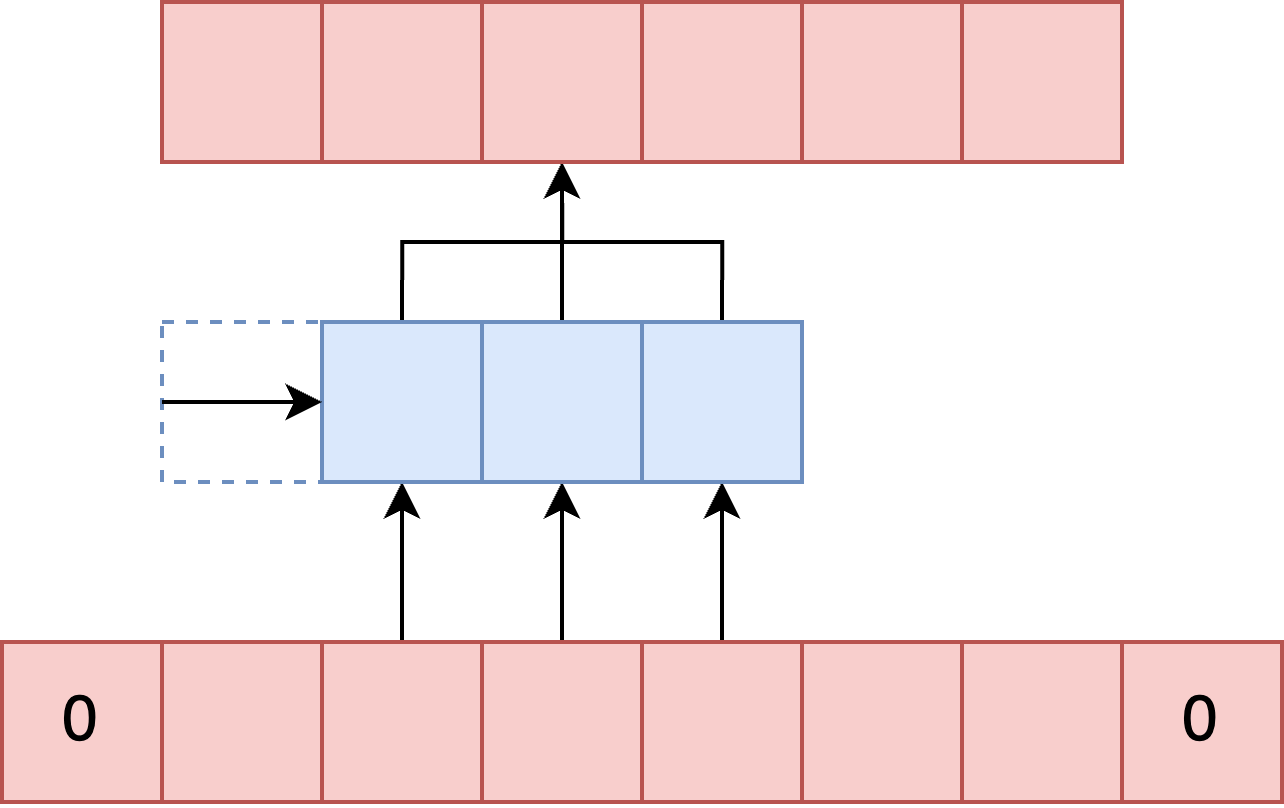
\includegraphics[height=4cm]{./figure/sec3/conv1.drawio.png}
        \caption{$\lr{\kernelSizeUpper, \strideUpper, \dilationUpper} = \lr{3, 1, 1}$}
        \label{sec3:fig:conv1}
    \end{subfigure}
    \begin{subfigure}[b]{0.48\textwidth}
        \centering
        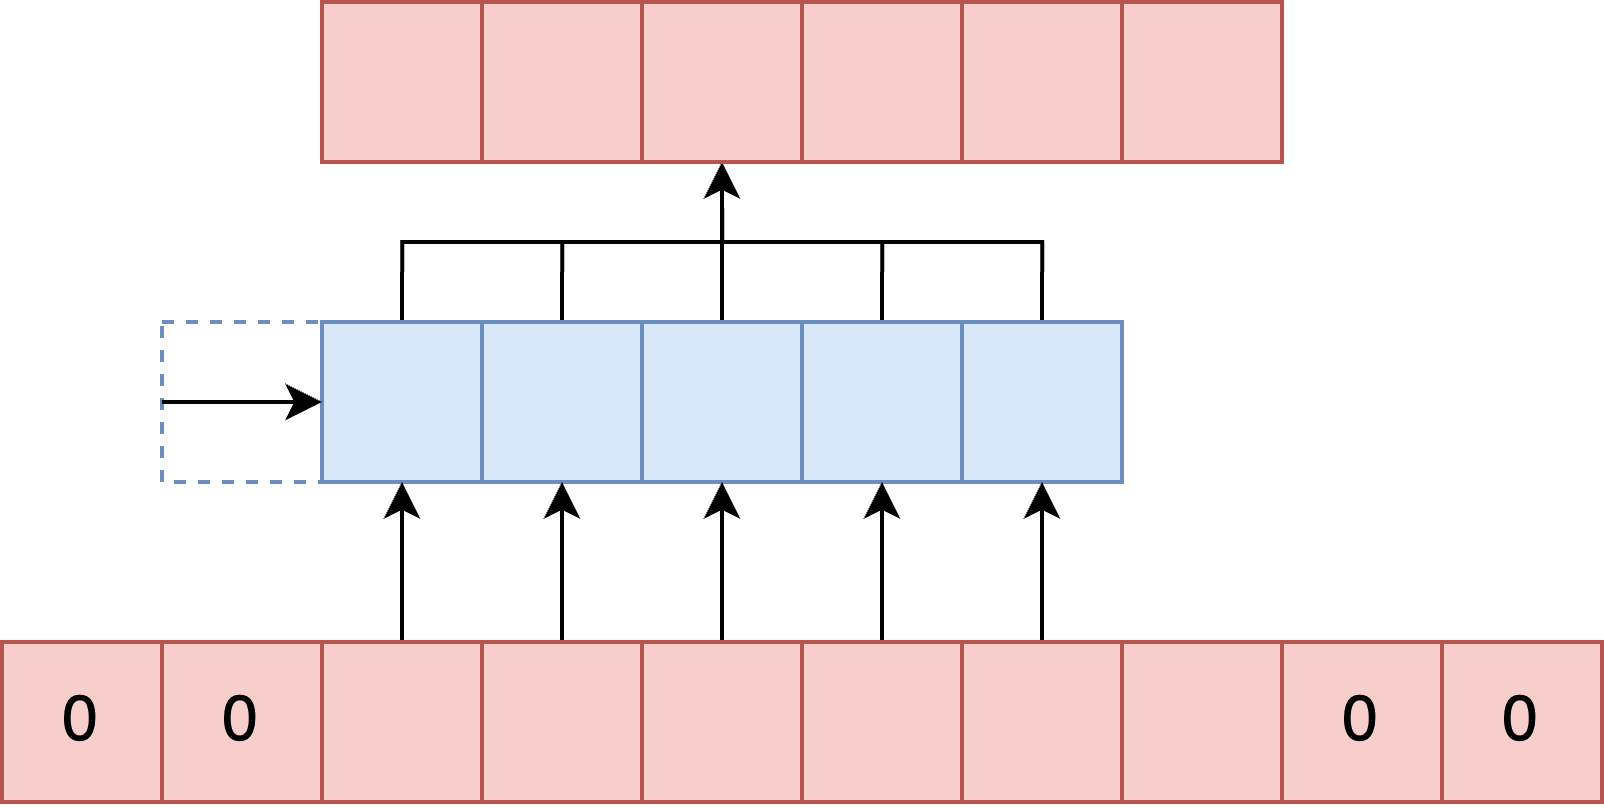
\includegraphics[height=4cm]{./figure/sec3/conv2.drawio.png}
        \caption{$\lr{\kernelSizeUpper, \strideUpper, \dilationUpper} = \lr{5, 1, 1}$}
        \label{sec3:fig:conv2}
    \end{subfigure}

    \vspace{0.5cm}

    \begin{subfigure}[b]{0.48\textwidth}
        \centering
        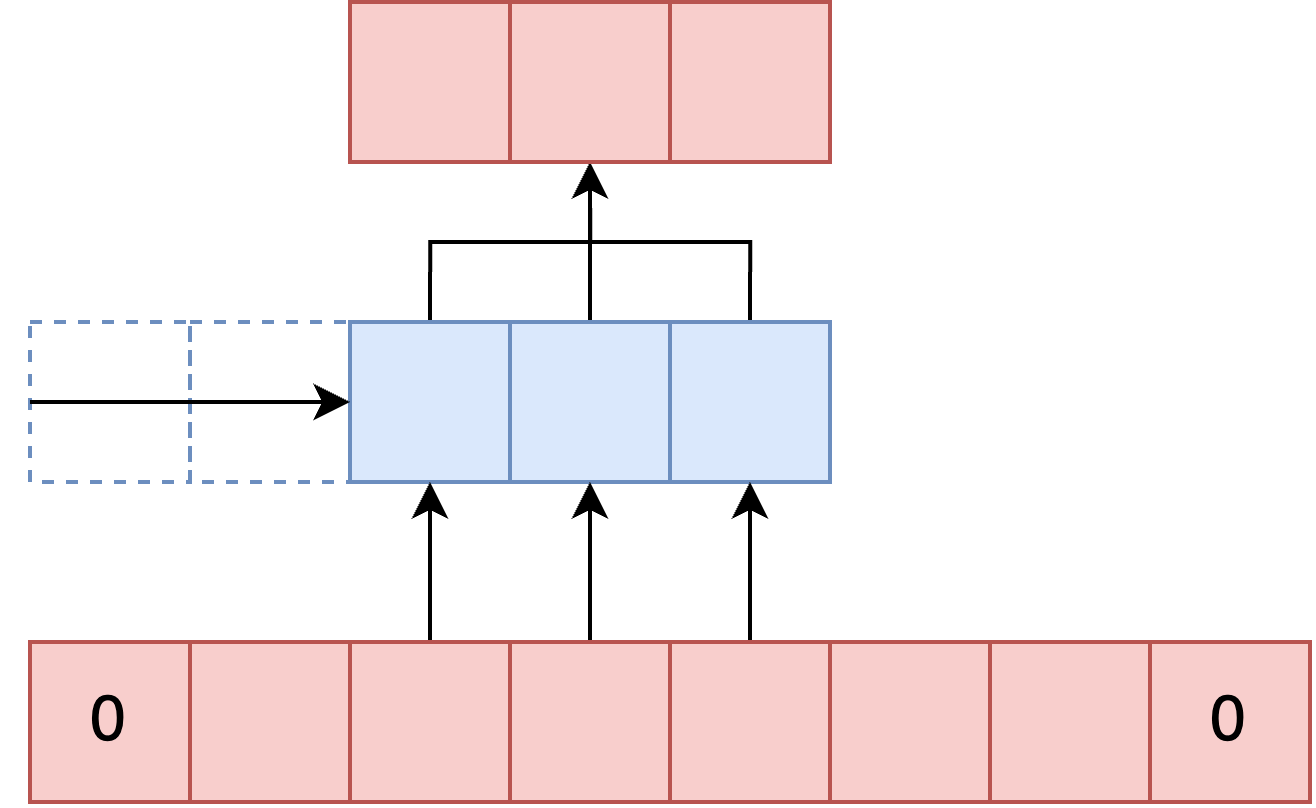
\includegraphics[height=4cm]{./figure/sec3/conv3.drawio.png}
        \caption{$\lr{\kernelSizeUpper, \strideUpper, \dilationUpper} = \lr{3, 2, 1}$}
        \label{sec3:fig:conv3}
    \end{subfigure}
    \begin{subfigure}[b]{0.48\textwidth}
        \centering
        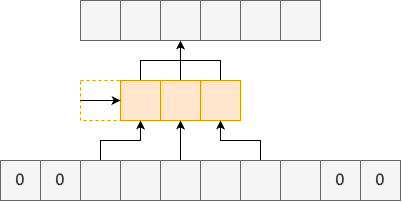
\includegraphics[height=4cm]{./figure/sec3/conv4.drawio.png}
        \caption{$\lr{\kernelSizeUpper, \strideUpper, \dilationUpper} = \lr{3, 1, 2}$}
        \label{sec3:fig:conv4}
    \end{subfigure}
    \caption{ある次元における一次元畳み込み層の処理.$\kernelSizeUpper$はカーネルサイズ,$\strideUpper$はストライド,$\dilationUpper$はダイレーションを表し,図中の0はパディング部を表す.}
    \label{sec3:fig:conv_variations}
\end{figure}

\subsubsection{転置畳み込み層}
転置畳み込み層は,畳み込み層の逆演算に対応する層であり,主に入力のアップサンプリングに使用される.図~\ref{sec3:fig:tconv_variations}に,ある入出力次元間における一次元転置畳み込み層の処理を示す.一次元転置畳み込み層では,$\timeLower$番目の入力とカーネルの積を計算し,その結果を$\timeLower$番目から$\timeLower + \kernelSizeUpper$番目までの出力とする.ここで$\kernelSizeUpper$はカーネルサイズである.また,複数の入力から計算された出力がオーバーラップする場合,これらは加算される.図~\ref{sec3:fig:tconv1}は,カーネルサイズを4,ストライドを1とした場合の様子である.アップサンプリングを行いたい場合は,ストライドを2以上とすれば良い.図~\ref{sec3:fig:tconv2}にカーネルサイズを4,ストライドを2とした場合を示す.この時,入力系列長が4であるのに対して,出力系列長が10まで拡大されていることがわかる.ここで,出力系列長を入力系列長の整数倍に保つためには,出力の両端の削除数を適切に設定する必要がある.上述の例では両端の削除数を1とすることで,出力系列長を入力系列長の2倍である8に調整できる.

\begin{figure}[tb]
    \centering
    \begin{subfigure}[b]{0.48\textwidth}
        \centering
        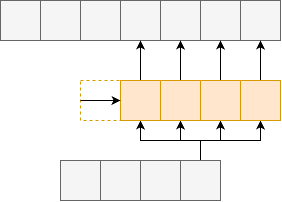
\includegraphics[height=4cm]{./figure/sec3/tconv1.drawio.png}
        \caption{$\lr{\kernelSizeUpper, \strideUpper} = \lr{4, 1}$}
        \label{sec3:fig:tconv1}
    \end{subfigure}
    \begin{subfigure}[b]{0.48\textwidth}
        \centering
        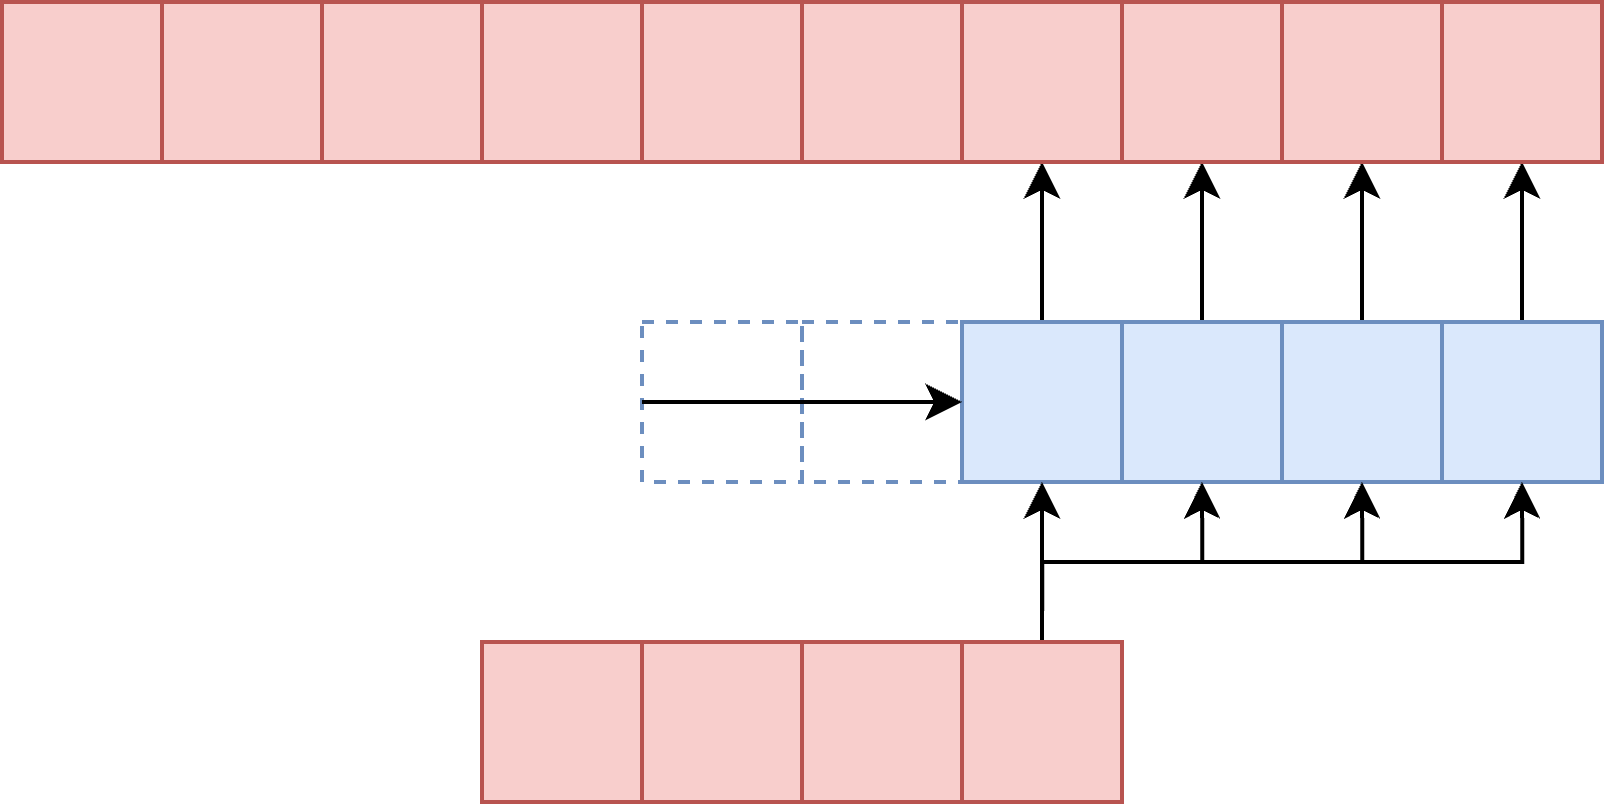
\includegraphics[height=4cm]{./figure/sec3/tconv2.drawio.png}
        \caption{$\lr{\kernelSizeUpper, \strideUpper} = \lr{4, 2}$}
        \label{sec3:fig:tconv2}
    \end{subfigure}
    \caption{ある次元における一次元転置畳み込み層の処理.$\kernelSizeUpper$はカーネルサイズ,$\strideUpper$はストライドを表す.}
    \label{sec3:fig:tconv_variations}
\end{figure}

\subsubsection{活性化関数}
活性化関数は,ニューラルネットワークの出力に非線形性を与えるための関数である.これにより,DNNは単純な線形変換だけでは表現できない複雑な入出力の関係を学習可能になる.以下,活性化関数への入力を$\inputLower \in \realSet$として,代表的なものを六つ述べる.また,本節で取り上げる活性化関数とその一階導関数のグラフを図~\ref{sec3:fig:activations_and_their_prime}に示す.

一つ目は,シグモイド関数である.シグモイド関数は
\begin{equation}
    \sigmoid\lr{\inputLower} = \frac{1}{1 + \exp\lr{-\inputLower}}
\end{equation}
で与えられ,その一階導関数は
\begin{equation}
    \dv{\sigmoid\lr{\inputLower}}{x} = \frac{\exp\lr{-\inputLower}}{\lr{1 + \exp\lr{-\inputLower}}^{2}}
\end{equation}
となる.図~\ref{sec3:fig:activations_prime}より,シグモイド関数の一階導関数の最大値は$\inputLower=0$における0.25であり,$\lrAbs{\inputLower - 0}$が大きくなるのに伴ってその値は小さくなることがわかる.DNNの各重みは,損失関数の勾配を利用することで更新されるから,シグモイド関数以前の層の重みにおける勾配は,シグモイド関数の一階導関数の値が乗算された結果となる.前述したように,シグモイド関数は一階導関数の値が小さくなりがちであるから,それ以前の層における勾配も小さくなり,重みの更新が進みづらくなる可能性がある.この問題を,勾配消失と呼ぶ.

二つ目は,$\tanh$関数である.$\tanh$は
\begin{equation}
    \tanh\lr{\inputLower} = \frac{\exp\lr{\inputLower} - \exp\lr{-\inputLower}}{\exp\lr{\inputLower} + \exp\lr{-\inputLower}}
\end{equation}
で与えられ,その一階導関数は
\begin{align}
    \dv{\tanh\lr{\inputLower}}{x} & = \frac{4}{\lr{\exp\lr{\inputLower} + \exp\lr{-\inputLower}}^{2}} \\
                                  & = \frac{1}{\cosh\lr{\inputLower}^{2}}
\end{align}
となる.$\tanh$の値域は$\lrClosedInterval{-1}{1}$となっており,図\ref{sec3:fig:activations_prime}より$\lrAbs{\inputLower - 0}$が小さいところではシグモイド関数より一階導関数の値が大きくなっていることがわかる.しかし,$\lrAbs{\inputLower - 0}$が大きくなればシグモイド関数と同様に一回導関数の値が小さく,勾配消失のリスクを抱えていることがわかる.

三つ目は,$\relu$である.$\relu$は
\begin{equation}
    \relu\lr{\inputLower} = \max \lr{0, \inputLower}
\end{equation}
で与えられ,その一階導関数は
\begin{equation}
    \dv{\relu\lr{\inputLower}}{x} =
    \begin{cases}
        1 & \text{if $\inputLower > 0$}  \\
        0 & \text{if $\inputLower <= 0$}
    \end{cases}
\end{equation}
となる.ここで,$\relu$は本来$x = 0$で微分不可能であるが,便宜上$\dv*{\relu\lr{0}}{x} = 0$とした.$\relu$は入力が0以上であれば恒等写像として振る舞うが,0未満であれば0に写す.一階導関数は0あるいは1のみを取り,特に入力が正の値であれば常に微分係数は1となることから,シグモイド関数や$\tanh$よりも勾配消失が起こりづらい.$\relu$は現在,標準的な活性化関数として広く用いられている.しかし,$\relu$への入力が0未満の値を取るとき,$\relu$入力についての出力の勾配は0になるから,$\relu$以前の層の重みが更新されず,学習が遅くなる可能性がある.

四つ目は,$\leakyRelu$\cite{maas2013rectifier}である.$\leakyRelu$は
\begin{equation}
    \leakyRelu\lr{\inputLower} =
    \begin{cases}
        \inputLower  & \text{if $\inputLower > 0$}  \\
        a\inputLower & \text{if $\inputLower <= 0$}
    \end{cases}
\end{equation}
で与えられ,その一階導関数は
\begin{equation}
    \dv{\leakyRelu\lr{\inputLower}}{x} =
    \begin{cases}
        1 & \text{if $\inputLower > 0$}  \\
        a & \text{if $\inputLower <= 0$}
    \end{cases}
\end{equation}
となる.ここで,$\leakyRelu$は本来$x = 0$で微分不可能であるが,便宜上$\dv*{\leakyRelu\lr{0}}{x} = a$とした.ReLUと比較すると,0未満の入力に対しても0でない値を出力し,一階導関数も0にならない点が異なっている.これにより,重みの更新が進まなくなるReLUの課題を解消した.

五つ目は,$\prelu$\cite{he2015delving}である.これは,$\leakyRelu$と似た活性化関数であるが,$\leakyRelu$のパラメータ$a$を学習可能にすることで,その他の層と合わせて最適化が可能となったことが特徴である.

六つ目は,$\gelu$\cite{hendrycks2016gaussian}である.$\gelu$は
\begin{equation}
    \gelu\lr{\inputLower} = \inputLower \Phi\lr{\inputLower}
\end{equation}
で与えられる.ここで,
\begin{equation}
    \Phi\lr{\inputLower} = P\lr{X \le \inputLower}, ~ X \sim \mathcal{N} \lr{0, 1}
\end{equation}
である.$\gelu$の一階導関数は,
\begin{equation}
    \dv{\gelu\lr{\inputLower}}{x} = \Phi\lr{\inputLower} + \frac{\inputLower}{\sqrt{2\pi}}\exp\lr{-\frac{\inputLower^{2}}{2}}
\end{equation}
となる.$\gelu$は,$\relu$が入力に対して0あるいは1を確定的にかける活性化関数と捉えた上で,これを入力に依存した確率的な挙動に変更したものである.実際,$\binaryMaskLower \sim \text{Bernoulli}\lr{\Phi\lr{\inputLower}}$とすると,
\begin{align}
    \gelu\lr{\inputLower} & = \inputLower \Phi\lr{\inputLower}                                                             \\
                          & = 1 \inputLower \cdot \Phi\lr{\inputLower} + 0 \inputLower \cdot \lr{1 - \Phi\lr{\inputLower}} \\
                          & = \expectation{mx}
\end{align}
となり,$\gelu$の出力は確率的なバイナリマスク$\binaryMaskLower$を入力$\inputLower$にかけた,$mx$の期待値に等しいことがわかる.

\begin{figure}[tb]
    \centering
    \begin{subfigure}[b]{1.0\textwidth}
        \centering
        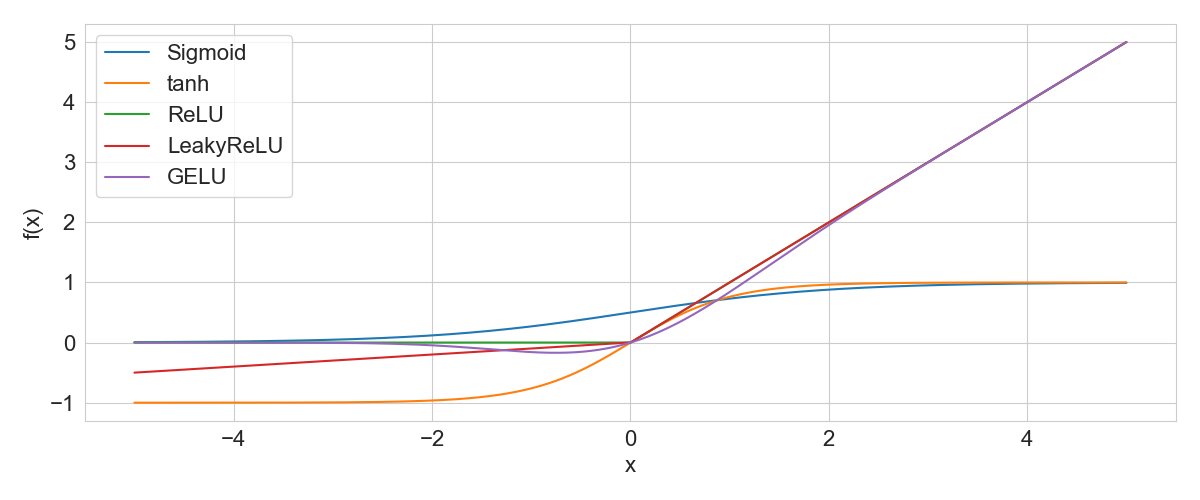
\includegraphics[height=6cm]{./figure/sec3/activations.png}
        \caption{活性化関数}
        \label{sec3:fig:activations}
    \end{subfigure}
    \begin{subfigure}[b]{1.0\textwidth}
        \centering
        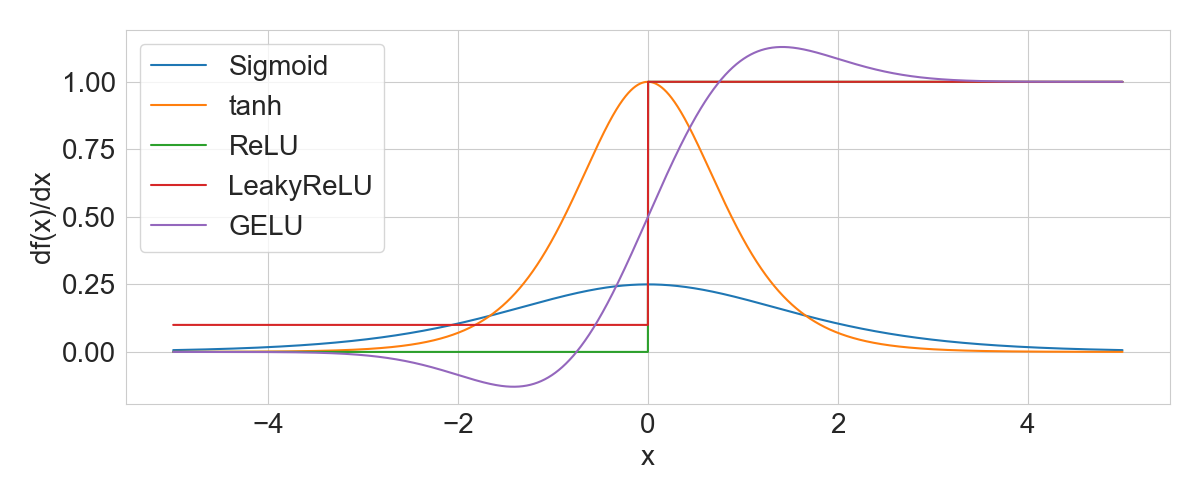
\includegraphics[height=6cm]{./figure/sec3/activations_prime.png}
        \caption{活性化関数の一階導関数}
        \label{sec3:fig:activations_prime}
    \end{subfigure}
    \caption{活性化関数の例}
    \label{sec3:fig:activations_and_their_prime}
\end{figure}

\subsubsection{再帰型ニューラルネットワーク}
再帰型ニューラルネットワーク(Recurrent Neural Network; RNN)は,自身の過去の出力を保持し,それをループさせる再帰的な構造を持ったネットワークである.

近年よく用いられるRNNとして,長・短期記憶(Long Short-Time Memory; LSTM)\cite{hochreiter1997long}がある.LSTMは入力ゲート,忘却ゲート,出力ゲートの3つを持ち,これらゲートによってネットワーク内部の情報の取捨選択を行うことで,長い系列データからの学習を可能にした.LSTMのネットワーク内部で行われる計算を以下に示す.
% concatTwo
\begin{gather}
    \bm{f}_{\timeLower} = \sigmoid\lr{\bm{\weightUpper}_{f}\concat{\bm{\inputLower}_{\timeLower}, \bm{h}_{\timeLower-1}} + \bm{\biasLower}_{f}} \\
    \bm{i}_{\timeLower} = \sigmoid\lr{\bm{\weightUpper}_{i}\concat{\bm{\inputLower}_{\timeLower}, \bm{h}_{\timeLower-1}} + \bm{\biasLower}_{i}} \\
    \tilde{\bm{c}}_{\timeLower} = \tanh\lr{\bm{\weightUpper}_{h}\concat{\bm{\inputLower}_{\timeLower}, \bm{h}_{\timeLower-1} + \bm{\biasLower}_{h}}} \\
    \bm{c}_{\timeLower} = \bm{f}_{\timeLower} \elemMul \bm{c}_{\timeLower-1} + \bm{i}_{\timeLower} \elemMul \tilde{\bm{c}}_{\timeLower} \\
    \bm{o}_{\timeLower} = \sigmoid\lr{\bm{\weightUpper}_{o}\concat{\bm{\inputLower}_{\timeLower}, \bm{h}_{\timeLower-1}} + \bm{\biasLower}_{o}} \\
    \bm{h}_{\timeLower} = \bm{o}_{\timeLower} \elemMul \tanh\lr{\bm{c}_{\timeLower}}
\end{gather}
ここで,$\bm{\inputLower}_{\timeLower} \in \realSet^{\dimUpper_{\text{in}}}$は時刻$\timeLower$の入力,$\bm{f}_{\timeLower} \in \lrsq{0, 1}^{\dimUpper_{\text{out}}}$は忘却ゲートの出力,$\bm{i}_{\timeLower} \in \lrsq{0, 1}^{\dimUpper_{\text{out}}}$は入力ゲートの出力,$\bm{c}_{\timeLower} \in \lrsq{-1, 1}^{\dimUpper_{\text{out}}}$が時刻$\timeLower$におけるセルの状態,$\bm{o}_{\timeLower} \in \lrsq{0, 1}^{\dimUpper_{\text{out}}}$が出力ゲートの出力,$\bm{h}_{\timeLower} \in \lrsq{-1, 1}^{\dimUpper_{\text{out}}}$が時刻$\timeLower$における隠れ状態を表す.$\bm{\weightUpper}_{f}, \bm{\weightUpper}_{i}, \bm{\weightUpper}_{h}, \bm{\weightUpper}_{o} \in \realSet^{\dimUpper_{\text{out}} \times \lr{\dimUpper_{\text{in}} + \dimUpper_{\text{out}}}}$は重み,$\bm{\biasLower}_{f}, \bm{\biasLower}_{i}, \bm{\biasLower}_{h}, \bm{\biasLower}_{o} \in \realSet^{\dimUpper_{\text{out}}}$はバイアスである.忘却ゲート出力$\bm{f}_{\timeLower}$が前時刻のセル状態$\bm{c}_{\timeLower}$に含まれる情報の選択,入力ゲート出力$\bm{i}_{\timeLower}$が新たな入力$\tilde{\bm{c}}_{\timeLower}$に含まれる情報の選択に用いられ,$\bm{c}_{\timeLower}$が決まる.その後,出力ゲート出力$\bm{o}_{\timeLower}$が$\bm{c}_{\timeLower}$に含まれる情報の選択に用いられ,$\bm{h}_{\timeLower}$が決まる.

また,LSTMが3つのゲートを必要とするのに対し,ゲートを2つに減らすことでネットワークの軽量化を図ったのがゲート付き回帰型ユニット(Gated Recurrent Unit; GRU)\cite{cho2014learning}である.GRUはリセットゲートと更新ゲートの2つを用いて隠れ状態を更新する.GRUのネットワーク内部で行われる計算を以下に示す.
\begin{gather}
    \bm{z}_{\timeLower} = \sigmoid\lr{\bm{\weightUpper}_{z}\concat{\bm{x}_{\timeLower}, \bm{h}_{\timeLower-1}} + \bm{\biasLower}_{z}} \\
    \bm{r}_{\timeLower} = \sigmoid\lr{\bm{\weightUpper}_{r}\concat{\bm{x}_{\timeLower}, \bm{h}_{\timeLower-1}} + \bm{\biasLower}_{r}} \\
    \tilde{\bm{h}}_{\timeLower} = \tanh\lr{\bm{\weightUpper}_{h}\concat{\bm{x}_{\timeLower}, \bm{r}_{\timeLower} \elemMul \bm{h}_{\timeLower-1}} + \bm{\biasLower}_{h}} \\
    \bm{h}_{\timeLower} = \lr{1 - \bm{z}_{\timeLower}} \elemMul \bm{h}_{\timeLower-1} + \bm{z}_{\timeLower} \elemMul \tilde{\bm{h}}_{\timeLower}
\end{gather}
ここで,$\bm{x}_{\timeLower} \in \realSet^{\dimUpper_{\text{in}}}$が時刻$\timeLower$における入力,$\bm{z}_{\timeLower} \in \lrsq{0, 1}^{\dimUpper_{\text{out}}}$が更新ゲートの出力,$\bm{r}_{\timeLower} \in \lrsq{0, 1}^{\dimUpper_{\text{out}}}$がリセットゲートの出力,$\bm{h}_{\timeLower} \in \lrsq{-1, 1}^{\dimUpper_{\text{out}}}$が時刻$\timeLower$における隠れ状態を表す.また,$\bm{\weightUpper}_{z}, \bm{\weightUpper}_{r}, \bm{\weightUpper}_{h} \in \realSet^{\dimUpper_{\text{out}} \times \lr{\dimUpper_{\text{in}} + \dimUpper_{\text{out}}}}$は重み,$\bm{\biasLower}_{z}, \bm{\biasLower}_{r}, \bm{\biasLower}_{h} \in \realSet^{\dimUpper_{\text{out}}}$はバイアスである.更新ゲート出力$\bm{z}_{\timeLower}$が$\bm{h}_{\timeLower - 1}$と$\tilde{\bm{h}}_{\timeLower}$に含まれる情報の選択,リセットゲート出力$\bm{r}_{\timeLower}$が$\bm{h}_{\timeLower - 1}$に含まれる情報の選択に用いられる.

\subsubsection{正規化層}
DNNの学習過程では学習の進行に伴って重みが変化するため,その度に各層への入力の分布が変わってしまう.これは内部共変量シフトと呼ばれ,ネットワークの学習を不安定にする原因となる.これに対し,バッチ正規化(Batch Normalization)\cite{ioffe2015batch}が有効である.バッチ正規化は,ミニバッチ内における入力特徴量の期待値と分散を次元ごとに計算し,これらを用いて入力特徴量を次元ごとに標準化するものである.ここで,バッチサイズを$\numUpper$,バッチ正規化への入力特徴量を$\bm{\inputLower}_{\numLower} \in \realSet^{\dimUpper} ~ \lr{\numLower = 1, \ldots, \numUpper}$,出力特徴量を$\bm{y}_{\numLower} \in \realSet^{\dimUpper} ~ \lr{\numLower = 1, \ldots, \numUpper}$とする.このとき,各$\numLower$に対し入力特徴量$\bm{\inputLower}_{\numLower}$の$\dimLower$次元目の成分を$\inputLower_{\numLower, \dimLower}$,出力特徴量$\bm{\outputLower}_{\numLower}$の$\dimLower$次元目の成分を$\outputLower_{\numLower, \dimLower}$とすると,$\outputLower_{\numLower, \dimLower}$は
\begin{align}
    \mean^{B}_{\dimLower}                      & = \frac{1}{\numUpper} \sum_{\numLower = 1}^{\numUpper} \inputLower_{\numLower, \dimLower}                                  \\
    \lr{\std^{B}_{\dimLower}}^{2}              & = \frac{1}{\numUpper} \sum_{\numLower = 1}^{\numUpper} \lr{\inputLower_{\numLower, \dimLower} - \mean^{B}_{\dimLower}}^{2} \\
    \tilde{\inputLower}_{\numLower, \dimLower} & = \frac{\inputLower_{\numLower, \dimLower} - \mean^{B}_{\dimLower}}{\sqrt{\lr{\std^{B}_{\dimLower}}^{2} + \epsilon}}       \\
    \outputLower_{\numLower, \dimLower}        & = \normScale_{\dimLower} \tilde{\inputLower}_{\numLower, \dimLower} +  \normShift_{\dimLower}
\end{align}
で与えられる.ここで,$\normScale_{\dimLower}, \normShift_{\dimLower} \in \realSet$は学習可能なスカラーであり,$\epsilon \in \realSet$はゼロ割を避けるためのスカラーである.バッチ正規化では$\normScale_{\dimLower}, \normShift_{\dimLower}$によって表現力を向上させており,実際
\begin{align}
    \normScale_{\dimLower} & = \sqrt{\lr{\std^{B}_{\dimLower}}^{2} + \epsilon} \\
    \beta_{\dimLower}      & = \mean^{B}_{\dimLower}
\end{align}
とすれば,標準化前の入力を再び得ることが可能である.学習時は,サンプルの標準化に用いる統計量とは別に,期待値の移動平均と不偏分散の移動平均を計算しておく.推論時は学習終了時に得られたこれら移動平均の値を用いることで,確率的な挙動を持たないよう工夫されている.

バッチ正規化はDNNの学習の安定化に貢献する一方,ミニバッチ全体における統計量を利用するため,バッチサイズが小さい場合はデータの分布を安定させることが難しくなる.また,テキストや音声といった系列長を持つデータを扱う場合,ミニバッチを構成するためにはゼロパディングによって系列長を揃える必要がある.この時,RNNの各ステップの出力に対しバッチ正規化を適用すると,ゼロパディングによって人為的に系列量を揃えているから,統計量が実際のデータの分布からかけ離れたものになる可能性がある.これら課題に対し,ミニバッチ内の各サンプルごとに期待値と分散を求めて標準化する,レイヤー正規化(Layer Normalization)\cite{ba2016layer}がある.バッチ正規化のときと同様の表記を用いると,$\outputLower_{\numLower, \dimLower}$は
\begin{align}
    \mean^{L}_{\numLower}                      & = \frac{1}{\dimUpper} \sum_{\dimLower = 1}^{\dimUpper} \inputLower_{\numLower, \dimLower}                                  \\
    \lr{\std^{L}_{\numLower}}^{2}              & = \frac{1}{\dimUpper} \sum_{\dimLower = 1}^{\dimUpper} \lr{\inputLower_{\numLower, \dimLower} - \mean^{L}_{\numLower}}^{2} \\
    \tilde{\inputLower}_{\numLower, \dimLower} & = \frac{\inputLower_{\numLower, \dimLower} - \mean^{L}_{\numLower}}{\sqrt{\lr{\std^{L}_{\numLower}}^{2} + \epsilon}}       \\
    \outputLower_{\numLower, \dimLower}        & = \normScale_{\dimLower} \tilde{\inputLower}_{\numLower, \dimLower} +  \normShift_{\dimLower}
\end{align}
で与えられる.

上述したバッチ正規化およびレイヤー正規化は,特徴量を標準化することで学習を安定させる手法であった.一方,DNN内のある層の重みを再パラメータ化することで学習を安定させる手法として,重み正規化(Weight Normalization)\cite{salimans2016weight}がある.これは,ある層の重みベクトル$\bm{\weightLower}$を,
\begin{equation}
    \bm{\weightLower} = \frac{\bm{v}}{\lrOneNorm{\bm{v}}} g
\end{equation}
のように単位ベクトル$\bm{v} / \lrOneNorm{\bm{v}}$(ベクトルの向き)とスカラー$g$(ベクトルの大きさ)に再パラメータ化するものである.学習時は重みの更新を$\bm{v}$と$g$で別々に行う.重み正規化は,バッチ正規化やレイヤー正規化と同様に学習の安定化に役立つが,計算に入力特徴量の系列長が依存しない.そのため,例えば音声波形など系列長が非常に長くなりがちなデータを扱う場合,計算コストを下げながら同様の効果を狙える手段だと考えられる.

\subsubsection{Transformer}
Transformer\cite{vaswani2017attention}は,自己注意機構(Self-Attention)を用いて,入力系列全体に渡る依存関係を捉えることができるニューラルネットワークである.特に,再帰的な計算を必要とするRNNと比較して,Transformerは並列計算のみ行うため,GPUによる計算の高速化が可能である.以下,入力特徴量を$\bm{\inputUpper} \in \realSet^{\timeUpper \times \dimUpper_{\text{model}}}$として,Transformerにおいて行われる計算を説明する.また,Transformer層の構造を図~\ref{sec3:fig:transformer_layer}に示す.

\begin{figure}[bt]
    \centering
    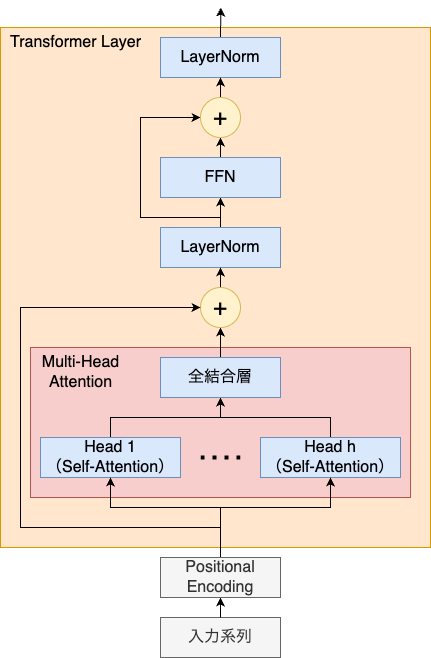
\includegraphics[height=140mm]{./figure/sec3/transformer.drawio.png}
    \caption{Transformer層の構造}
    \label{sec3:fig:transformer_layer}
\end{figure}

まず,TransformerにおけるSelf-Attentionの計算の流れを述べる.ここでは,はじめにクエリ$\bm{Q} \in \realSet^{\timeUpper \times \dimUpper_{k}}$,キー$\bm{K} \in \realSet^{\timeUpper \times \dimUpper_{k}}$,バリュー$\bm{V} \in \realSet^{\timeUpper \times \dimUpper_{v}}$の計算を行う.これは,
\begin{align}
    \bm{Q} & = \bm{\inputUpper}\bm{\weightUpper}_{Q} + \lrRepeatTr{\bm{\biasLower}_{Q}}{T} \\
    \bm{K} & = \bm{\inputUpper}\bm{\weightUpper}_{K} + \lrRepeatTr{\bm{\biasLower}_{K}}{T} \\
    \bm{V} & = \bm{\inputUpper}\bm{\weightUpper}_{V} + \lrRepeatTr{\bm{\biasLower}_{V}}{T}
\end{align}
で与えられる.ここで,$\bm{\weightUpper}_{Q}, \bm{\weightUpper}_{K} \in \realSet^{\dimUpper_{\text{model}} \times \dimUpper_{k}}, \bm{\weightUpper}_{V} \in \realSet^{\dimUpper_{\text{model}} \times \dimUpper_{v}}$は重み,$\bm{\biasLower}_{Q}, \bm{\biasLower}_{K} \in \realSet^{\dimUpper_{k}}, \bm{\biasLower}_{V} \in \realSet^{\dimUpper_{v}}$はバイアスである.また,$\lrRepeat{\bm{\biasLower}_{Q}}{T} \in \realSet^{\dimUpper_{k} \times \timeUpper}$は,列ベクトル$\bm{\biasLower}_{Q}$を$T$回列方向に並べる操作を表す.

次に,クエリとキーを元にアテンション重みを求め,バリューに対する行列積を計算する.これは,
\begin{equation}
    \text{Attention}\lr{\bm{Q}, \bm{K}, \bm{V}} = \text{softmax}\lr{\frac{\bm{Q}\bm{K}^\top}{\sqrt{\dimUpper_{k}}}} \bm{V}
\end{equation}
で与えられる.softmax関数は行方向に適用されるため,$\text{softmax}\lr{\bm{Q}\bm{K}^\top / \sqrt{\dimUpper_{k}}}$の各行ベクトルが,各クエリ$\bm{q}_{t} \in \realSet^{\dimUpper_{k}}$からキー$\bm{k}_{t} \in \realSet^{\dimUpper_{k}}, ~ \lr{t = 1, \ldots, T}$に対する注意度になっている.

ここまでがSelf-Attentionの計算であったが,TransformerではSelf-Attentionを複数のヘッドで並列に計算し,各ヘッドの出力を結合して最終出力を得るMulti-Head Attentionが採用されている.ヘッド数を$\numHeadUpper$とすると,各ヘッド$\numHeadLower$におけるクエリ$\bm{Q}^{\numHeadLower} \in \realSet^{\timeUpper \times \frac{\dimUpper_{k}}{\numHeadUpper}}$,キー$\bm{K}^{\numHeadLower} \in \realSet^{\timeUpper \times \frac{\dimUpper_{k}}{\numHeadUpper}}$,バリュー$\bm{V}^{\numHeadLower} \in \realSet^{\timeUpper \times \frac{\dimUpper_{v}}{\numHeadUpper}}$の計算は,
\begin{align}
    \bm{Q}^{\numHeadLower} & = \bm{\inputUpper}\bm{\weightUpper}_{Q}^{\numHeadLower} + \lrRepeatTr{\bm{\biasLower}_{Q}^{\numHeadLower}}{T} \\
    \bm{K}^{\numHeadLower} & = \bm{\inputUpper}\bm{\weightUpper}_{K}^{\numHeadLower} + \lrRepeatTr{\bm{\biasLower}_{K}^{\numHeadLower}}{T} \\
    \bm{V}^{\numHeadLower} & = \bm{\inputUpper}\bm{\weightUpper}_{V}^{\numHeadLower} + \lrRepeatTr{\bm{\biasLower}_{V}^{\numHeadLower}}{T}
\end{align}
で与えられる.ここで,$\bm{\weightUpper}_{Q}^{\numHeadLower}, \bm{\weightUpper}_{K}^{\numHeadLower} \in \realSet^{\dimUpper_{\text{model}} \times \frac{\dimUpper_{k}}{\numHeadUpper}}$,$\bm{\weightUpper}_{V}^{\numHeadLower} \in \realSet^{\dimUpper_{\text{model}} \times \frac{\dimUpper_{v}}{\numHeadUpper}}$は重み,$\bm{\biasLower}_{Q}^{\numHeadLower}, \bm{\biasLower}_{K}^{\numHeadLower} \in \realSet^{\frac{\dimUpper_{k}}{\numHeadUpper}}, \bm{\biasLower}_{V}^{\numHeadLower} \in \realSet^{\frac{\dimUpper_{v}}{\numHeadUpper}}$はバイアスである.この後の処理もSelf-Attentionと同様に,
\begin{equation}
    \text{Attention}\lr{\bm{Q}^{\numHeadLower}, \bm{K}^{\numHeadLower}, \bm{V}^{\numHeadLower}} = \text{softmax}\lr{\frac{\bm{Q}^{\numHeadLower}\lr{\bm{K}^{\numHeadLower}}^\top}{\sqrt{\dimUpper_{k}} / \numHeadUpper}} \bm{V}^{\numHeadLower}
\end{equation}
となる.ここで得られた各ヘッドからの出力を結合し,さらに全結合層を通すことでMulti-Head Attetionの出力が得られる.すなわち,
\begin{equation}
    \text{MultiHead}\lr{\bm{Q}, \bm{K}, \bm{V}} = \concat{\text{Attention}\lr{\bm{Q}^{\numHeadLower}, \bm{K}^{\numHeadLower}, \bm{V}^{\numHeadLower}}, \ldots, \text{Attention}\lr{\bm{Q}^{\numHeadLower}, \bm{K}^{\numHeadLower}, \bm{V}^{\numHeadLower}}} \bm{\weightUpper}_{o} + \lrRepeatTr{\bm{\biasLower}_{o}}{T}
\end{equation}
と表される.ここで,$\bm{\weightUpper}_{o} \in \realSet^{\dimUpper_{v} \times \dimUpper_{\text{model}}}$は重み,$\bm{\biasLower}_{o} \in \realSet^{\dimUpper_{\text{model}}}$はバイアスである.ヘッドを分割して複数パターンのSelf-Attentionを可能にすることで,より複雑な入出力の関係を学習できると考えられる.Multi-Head Attention後は,残差結合とレイヤー正規化を適用する.すなわち,この出力$\bm{\outputUpper} \in \realSet^{\timeUpper \times \dimUpper_{\text{model}}}$は,
\begin{equation}
    \bm{\outputUpper} = \text{LayerNorm}\lr{\text{MultiHead}r{\bm{Q}, \bm{K}, \bm{V}} + \bm{\inputUpper}}
\end{equation}
で与えられる.その後,全結合層を通し,残差結合とレイヤー正規化を適用することでTransformer層最終出力を得る.すなわち,
\begin{equation}
    \bm{\outputUpper} = \text{LayerNorm}\lr{\lr{\relu\lr{\bm{\outputUpper}\bm{\weightUpper}_{1} + \lrRepeatTr{\bm{b}_{1}}{T}}\bm{\weightUpper}_{2} + \lrRepeatTr{\bm{b}_{2}}{T}} + \bm{\outputUpper}}
\end{equation}
となる.ここで,$\bm{\weightUpper}_{1} \in \realSet^{\dimUpper_{\text{model}} \times \dimUpper_{\text{fc}}}$,$\bm{\weightUpper}_{2} \in \realSet^{\dimUpper_{\text{fc}} \times \dimUpper_{\text{model}}}$は重み,$\bm{b}_{1} \in \realSet^{\dimUpper_{\text{fc}}}$,$\bm{b}_{2} \in \realSet^{\dimUpper_{\text{model}}}$はバイアスである.$\dimUpper_{\text{fc}}$は$\dimUpper_{\text{model}}$の4倍とされることが多い.Transformer全体は,Transformer層を多層積み重ねて構成される.

最後に,TransformerではRNNと違い,並列計算によって系列全体を一度に処理することが可能であるが,それと引き換えに入力の順序情報を考慮することができなくなる.これに対し,TransformerではPositional Encodingによって入力に位置情報を与える.Positional Encodingは$\sin$と$\cos$に基づいて,
\begin{equation}
    \text{PositionalEncoding}\lr{\timeLower, \dimLower} =
    \begin{cases}
        \sin \lr{\frac{\timeLower}{10000^{2\dimLower / \dimUpper_{\text{model}}}}} & \text{if $d \bmod 2 = 0$} \\
        \cos \lr{\frac{\timeLower}{10000^{2\dimLower / \dimUpper_{\text{model}}}}} & \text{if $d \bmod 2 = 1$}
    \end{cases}
\end{equation}
で与えられる.

\subsection{学習方法}
本節において,$\bm{\weightAndBias} \in \realSet^{\numUpper_{\text{model}}}$はDNNの重みとバイアスをまとめて表す変数とする.また,文章中では簡潔さを優先し,特別な理由がない限りは重みと呼ぶ.

\subsubsection{損失関数}
損失関数は,DNNによって推定された結果と正解値との間の誤差を求める関数のことであり,扱う問題によって様々である.例えば,回帰問題において用いられる関数の一つに,MAE(Mean Absolute Error)Lossがある.推定対象を$\bm{\outputLower} \in \realSet^{\dimUpper}$,DNNによる推定結果を$\hat{\bm{\outputLower}} \in \realSet^{\dimUpper}$とすると,MAE Lossは
\begin{equation}
    \lossFuncUpper_{\text{MAE}}\lr{\bm{\outputLower}, \hat{\bm{\outputLower}}} = \frac{1}{\dimUpper} \sum_{\dimLower = 1}^{\dimUpper}  |\outputLower_{\dimLower} - \hat{\outputLower}_{\dimLower}|
\end{equation}
で与えられる.また,推定対象が行列$\bm{\outputUpper} \in \realSet^{\dimUpper \times \timeUpper}$の場合,DNNによる推定結果を$\hat{\bm{\outputUpper}} \in \realSet^{\dimUpper \times \timeUpper}$とすると,
\begin{equation}
    \lossFuncUpper_{\text{MAE}}\lr{\bm{\outputUpper}, \hat{\bm{\outputUpper}}} = \frac{1}{\dimUpper \timeUpper} \sum_{\dimLower = 1}^{\dimUpper} \sum_{\timeLower = 1}^{\timeUpper}  |\outputLower_{\dimLower, \timeLower} - \hat{\outputLower}_{\dimLower, \timeLower}|
\end{equation}
で与えられる.

一方,分類問題において用いられる関数の一つに,Cross Entropy Lossがある.$\classUpper$クラス分類の問題について,推定対象を$\bm{\outputLower} \in \lrClosedInterval{0}{1}^{\classUpper}$,DNNによる推定結果を$\hat{\bm{\outputLower}} \in \realSet^{\classUpper}$とすると,Cross Entropy Lossは
\begin{equation}
    \lossFuncUpper_{\text{CE}}\lr{\bm{\outputLower}, \hat{\bm{\outputLower}}} = - \sum_{\classLower = 1}^{\classUpper} y_{\classLower} \log \frac{\exp\lr{\hat{\outputLower}_{c}}}{\sum_{i = 1}^{C} \exp\lr{\hat{\outputLower}_{c}}}
\end{equation}
で与えられる.ここで,$\bm{\outputLower}$はクラスに対する確率分布であり,
\begin{equation}
    \sum_{\classLower = 1}^{\classUpper} y_{\classLower} = 1
\end{equation}
を満たす.実際は,正解となるクラスのみを1,それ以外を0としたOne-hotベクトルとされることが多い.また,推定対象が行列$\bm{\outputUpper} \in \lrClosedInterval{0}{1}^{\classUpper}$の場合,DNNによる推定結果を$\hat{\bm{\outputUpper}} \in \realSet^{\classUpper \times \timeUpper}$とすると,
\begin{equation}
    \lossFuncUpper_{\text{CE}}\lr{\bm{\outputUpper}, \hat{\bm{\outputUpper}}} = - \frac{1}{\timeUpper} \sum_{\timeLower = 1}^{\timeUpper} \sum_{\classLower = 1}^{\classUpper} y_{\classLower, t} \log \frac{\exp\lr{\hat{\outputLower}_{\classLower, t}}}{\sum_{i = 1}^{C} \exp\lr{\hat{\outputLower}_{\classLower, t}}}
\end{equation}
で与えられる.

\subsubsection{勾配降下法}
\label{sec3:sec:gradient_descent}
勾配降下法(Gradient Descent)は,損失関数の重みについての勾配を利用して,損失関数の値を最小化するようにDNNを最適化するアルゴリズムである.ここで,学習データセットを$\dataset_{\text{train}} = \left\{\lr{\bm{\inputLower}_{\numLower}, \bm{\outputLower}_{\numLower}}\right\}_{\numLower = 1}^{\numUpper}$とする.各$n$に対し,$\bm{\inputLower}_{\numLower} \in \realSet^{\dimUpper_{\text{in}}}$はDNNへの入力, $\bm{\outputLower}_{\numLower} \in \realSet^{\dimUpper_{\text{out}}}$は予測対象を表す.DNNは$f: \realSet^{\dimUpper_{\text{in}}} \to \realSet^{\dimUpper_{\text{out}}}$で表し,予測値を$\hat{\bm{\outputLower}}_{\numLower} = f\lr{\bm{\inputLower}_{\numLower}; \bm{\weightAndBias}}$とする.損失関数は$\lossFuncUpper: \realSet^{\dimUpper_{\text{out}}} \times \realSet^{\dimUpper_{\text{out}}} \to \realSet$とし,$\mathcal{\lossFuncUpper}: \realSet^{\numUpper_{\text{model}}} \to \realSet$を,
\begin{equation}
    \mathcal{\lossFuncUpper}\lr{\bm{\weightAndBias}; \mathcal{\indexUpper}} = \frac{1}{|\mathcal{\indexUpper}|} \sum_{\indexLower \in \mathcal{\indexUpper}} \lossFuncUpper\lr{\bm{\outputLower}_{\indexLower}, \hat{\bm{\outputLower}}_{\indexLower}} = \frac{1}{|\mathcal{\indexUpper}|} \sum_{\indexLower \in \mathcal{\indexUpper}} \lossFuncUpper\lr{\bm{\outputLower}_{\indexLower}, f\lr{\bm{\inputLower}_{\indexLower}; \bm{\weightAndBias}}}
\end{equation}
で定義する.ここで,$\mathcal{\indexUpper} \subset \{1, \ldots, N\}$は各サンプルに対するインデックスの部分集合,$|\cdot|$は集合の元の数を表す.すなわち,$\mathcal{\lossFuncUpper}$は学習データ$\left\{\lr{\bm{\inputLower}_{\indexLower}, \bm{\outputLower}_{\indexLower}}\right\}_{\indexLower \in \indexUpper} \subset \mathcal{D}_{\text{train}}$に対する損失を,DNNの重み$\bm{\weightAndBias}$の関数として扱うものである.上の表記を用いれば,DNNの最適化問題は
\begin{equation}
    \min_{\bm{\weightAndBias} \in \realSet^{\numUpper_{\text{model}}}} \mathcal{\lossFuncUpper}\lr{\bm{\weightAndBias}; \{1, \ldots, N\}}
\end{equation}
と表される.この最適化問題に対し,勾配降下法による重み$\bm{\weightAndBias}$の更新は,
\begin{equation}
    \label{sec3:eq:normal_gradient_descent}
    \bm{\weightAndBias}_{\iter} = \bm{\weightAndBias}_{\iter - 1} - \learningRate \nabla_{\bm{\weightAndBias}} \mathcal{\lossFuncUpper}\lr{\bm{\weightAndBias}_{\iter - 1}; \mathcal{I}_{\iter}}
\end{equation}
で与えられる.ここで,$\iter \in \naturalSet$は学習におけるイテレーション,$\learningRate \in \lrLeftClosedInterval{0}{\infty}$は学習率を表す.

勾配降下法には,三種類の方法がある\cite{zhang2019gradient}.一つ目は,バッチ勾配降下法である.これは,
\begin{equation}
    \bm{\weightAndBias}_{\iter} = \bm{\weightAndBias}_{\iter - 1} - \learningRate \nabla_{\bm{\weightAndBias}} \mathcal{\lossFuncUpper}\lr{\bm{\weightAndBias}_{\iter - 1}; \{1, \ldots, N\}}
\end{equation}
で与えられる.すなわち,各イテレーションで学習データ全てを用いる方法である.各サンプルのノイズの影響が低減されることで安定した学習が期待できるが,計算コストが高い.二つ目は,確率的勾配降下法である.これは,ランダムに選択された$n_{\iter} \in \{1, \ldots, N\}$に対し,
\begin{equation}
    \bm{\weightAndBias}_{\iter} = \bm{\weightAndBias}_{\iter - 1} - \learningRate \nabla_{\bm{\weightAndBias}} \mathcal{\lossFuncUpper}\lr{\bm{\weightAndBias}_{\iter - 1}; \{n_{\iter}\}}
\end{equation}
で与えられる.すなわち,各イテレーションで単一サンプルのみを用いる方法である.計算コストが下がるが,各サンプルのノイズの影響が大きくなることで学習が不安定になる可能性がある.三つ目は,ミニバッチ勾配降下法である.これは,$1 < |\mathcal{I}_{\iter}| < N$を満たすランダムに選択された$\mathcal{I}_{\iter} \subsetneq \{1, \ldots, N\}$に対し,
\begin{equation}
    \bm{\weightAndBias}_{\iter} = \bm{\weightAndBias}_{\iter - 1} - \learningRate \nabla_{\bm{\weightAndBias}} \mathcal{\lossFuncUpper}\lr{\bm{\weightAndBias}_{\iter - 1}; \mathcal{I}_{\iter}}
\end{equation}
で与えられる.これより,各イテレーションで二つ以上のサンプルからなる学習データセットの真部分集合を用いる方法だと言える.バッチ勾配降下法と確率的勾配降下法の間をとった方法であり,DNNの学習においては一般にミニバッチ勾配降下法が用いられる.ここで,ミニバッチに含まれるサンプルの数をバッチサイズと呼ぶ.

また,確率的勾配降下法やミニバッチ勾配降下法では,サンプルを学習データセットからランダムに非復元抽出する.ここで,毎回のサンプリングされた学習データに対する処理は1イテレーションとカウントし,学習データセットを一度全て使い切ることは1エポックとカウントする.実際には,データセットの総サンプル数$N$に対してバッチサイズを決定することで1エポックあたりの総イテレーション数は決まり,最大エポック数を設定して学習を回すこととなる.

\subsubsection{正則化}
DNNは大量のパラメータにより高い表現力を持つが,その分学習データに過剰に適合し,未知データに対する汎化性能が低いモデルとなる,過学習を引き起こす可能性がある.正則化は,このようなDNNの過学習を防ぐための手段である.以下,具体的な方法を四つ述べる.

一つ目は,L2正則化である.これは,$\mathcal{\lossFuncUpper}\lr{\bm{\weightAndBias}; \mathcal{\indexUpper}}$を
\begin{equation}
    \label{sec3:eq:l2_reg}
    \mathcal{\lossFuncUpper}\lr{\bm{\weightAndBias}; \mathcal{\indexUpper}} = \frac{1}{|\mathcal{\indexUpper}|} \sum_{\indexLower \in \mathcal{\indexUpper}} \lossFuncUpper\lr{\bm{\outputLower}_{\indexLower}, f\lr{\bm{\inputLower}_{\indexLower}; \bm{\weightAndBias}}} + \frac{\regConst}{2} \lrTwoNorm{\bm{\weightAndBias}}^{2}
\end{equation}
とすることで与えられる.ここで,$\regConst \in \lrLeftClosedInterval{0}{\infty}$は正則化の程度を調整するパラメータである.これより,L2正則化は損失関数の値に$\lrTwoNorm{\bm{\weightAndBias}}^{2}$を加算することで,重み$\bm{\weightAndBias}$のL2ノルムが過大になることを防ぐ方法だと言える.

二つ目は,Weight Decayである.これは,重みの更新式を
\begin{equation}
    \label{sec3:eq:weight_decay}
    \bm{\weightAndBias}_{\iter} = \bm{\weightAndBias}_{\iter - 1} - \learningRate \nabla_{\bm{\weightAndBias}} \mathcal{\lossFuncUpper}\lr{\bm{\weightAndBias}_{\iter - 1}; \mathcal{I}_{\iter}} - \regConst' \bm{\weightAndBias}
\end{equation}
とすることで与えられる.ここで,$\regConst' \in \lrLeftClosedInterval{0}{\infty}$は正則化の程度を調整するパラメータである.これより,Weight Decayは重み$\bm{\weightAndBias}$の絶対値が過大になることを防ぐ手法だと言える.

三つ目は,Dropout\cite{srivastava2014dropout}である.Dropoutは,学習時に特徴量の一部を0に落とす手法である.一方,推論時は恒等写像となり,学習時と挙動が変わる.Dropoutへの入力を$\bm{\inputLower} \in \realSet^{\dimUpper_{\text{in}}}$,特徴量を0に落とす確率を$p \in \lr{0, 1}$とすると,学習時のDropout出力$\bm{\outputLower}_{\text{train}} \in \realSet^{\dimUpper_{\text{out}}}$および推論時のDropout出力$\bm{\outputLower}_{\text{infer}} \in \realSet^{\dimUpper_{\text{out}}}$は,
\begin{align}
    \bm{\outputLower}_{\text{train}} & = \frac{\bm{x} \elemMul \bm{m}}{1 - p} \label{sec3:eq:regularization_dropout_training_output} \\
    \bm{\outputLower}_{\text{infer}} & = \bm{x}
\end{align}
で与えられる.ここで,$\bm{m} \in \{0, 1\}^{\dimUpper_{\text{in}}}$は各成分$m_{\dimLower}$が確率$1 - p$で1,確率$p$で0をとる確率変数である.式\eqref{sec3:eq:regularization_dropout_training_output}より,学習時はDropout出力を$1 / \lr{1 - p}$倍していることがわかる.この理由は,学習時の出力の期待値と推論時の出力を一致させるためである.実際,確率変数$\bm{m}$の従う確率分布上で$\bm{\outputLower}_{\text{train}}$の期待値をとれば,
\begin{align}
    \expectation{\bm{\outputLower}_{\text{train}}} & = \expectation{\frac{\bm{x} \elemMul \bm{m}}{1 - p}}             \\
                                                   & = \frac{\bm{x}}{1 - p} \elemMul \expectation{\bm{m}}             \\
                                                   & = \frac{\bm{x}}{1 - p} \elemMul \lr{1 - p ~ \cdots ~ 1 - p}^\top \\
                                                   & = \bm{x} = \bm{\outputLower}_{\text{infer}}
\end{align}
となる.Dropoutは学習時に一部のニューロンを落とすことで,実質的に異なるネットワークを学習させていると考えることができる.よって,学習時の出力の期待値に推論時の出力を一致させることは,異なるネットワークから得られた出力の期待値をとり,アンサンブルモデルとして推論時の出力を得ていると解釈できる.

四つ目は,Early Stoppingである.Early Stoppingは,検証データに対する損失の増加を監視し,設定したエポック数だけ増加し続けた場合に学習を停止する手法である.これにより,学習データに対する過度なフィッティングを防止する.

\subsubsection{最適化手法}
% 時間あればadamがmomentamやrmspropの発展として解釈できることを述べても良い.
\label{sec3:sec:optimizer}
\ref{sec3:sec:gradient_descent}節において,DNNの重みが勾配降下法によって最適化されることを述べた.ここで,通常の勾配降下法に代わり,近年よく用いられる最適化手法としてAdam\cite{kingma2014adam}がある.Adamの計算過程をアルゴリズム\ref{sec3:algo:adam}に示す.ここで,$\bm{g}_{\iter} \in \realSet^{\numUpper_{\text{model}}}$は勾配の一次モーメント,$\bm{m}_{\iter} \in \realSet^{\numUpper_{\text{model}}}$が勾配の一次モーメントの指数移動平均,$\bm{v}_{\iter} \in \realSet^{\numUpper_{\text{model}}}$が勾配の二次モーメントの指数移動平均である.$\hat{\bm{m}}_{\iter}$および$\hat{\bm{v}}_{\iter}$はそれぞれ,$\bm{m}_{\iter}$および$\bm{v}_{\iter}$の初期値が0であることに起因するバイアスを防ぐための計算を行った結果である.また,$\optimEmaConst_{1}, \optimEmaConst_{2} \in \lrClosedInterval{0}{1}$が,指数移動平均の程度を調整するパラメータである.
\begin{algorithm}
    \caption{Adam}
    \label{sec3:algo:adam}
    \begin{algorithmic}[1]
        \State \textbf{Input:} $\learningRate$, $\optimEmaConst_{1}$, $\optimEmaConst_{2}$, $\regConst$, $\bm{\weightAndBias}_{0}$, $L\lr{\bm{\weightAndBias}}$
        \State \textbf{Initialize:} $\bm{m}_{0} = 0$, $\bm{v}_{0} = 0$
        \For{$\iter = 1$ to \texttt{...}}
        \State $\bm{g}_{\iter} = \nabla_{\bm{\weightAndBias}} \mathcal{\lossFuncUpper}\lr{\bm{\weightAndBias}_{\iter - 1}; \mathcal{I}_{\iter}} + \regConst \bm{\weightAndBias}_{\iter-1}$
        \State $\bm{m}_{\iter} = \optimEmaConst_{1} \bm{m}_{\iter-1} + \lr{1 - \optimEmaConst_{1}} \bm{g}_{\iter}$
        \State $\bm{v}_{\iter} = \optimEmaConst_{2} \bm{v}_{\iter-1} + \lr{1 - \optimEmaConst_{2}} \bm{g}_{\iter} \elemMul \bm{g}_{\iter}$
        \State $\tilde{\bm{m}}_{\iter} = \bm{m}_{\iter} / \lr{1 - \optimEmaConst_{1}^{\iter}}$
        \State $\tilde{\bm{v}}_{\iter} = \bm{v}_{\iter} / \lr{1 - \optimEmaConst_{2}^{\iter}}$
        \State $\bm{\weightAndBias}_{\iter} = \bm{\weightAndBias}_{\iter-1} - \learningRate \tilde{\bm{m}}_{\iter} / \lr{\sqrt{\tilde{\bm{v}}_{\iter}} + \epsilon}$
        \EndFor
        \State \textbf{Return} $\bm{\weightAndBias}_{\iter}$
    \end{algorithmic}
\end{algorithm}
ここで,Adamでは正則化としてL2正則化を採用したが,Weight Decayを採用した最適化手法としてAdamW\cite{loshchilov2017decoupled}がある.AdamWの計算過程をアルゴリズム\ref{sec3:algo:adamw}に示す.正則化がL2正則化からWeight Decayに変わった点以外は同じである.
\begin{algorithm}
    \caption{AdamW}
    \label{sec3:algo:adamw}
    \begin{algorithmic}[1]
        \State \textbf{Input:} $\learningRate$, $\optimEmaConst_{1}$, $\optimEmaConst_{2}$, $\regConst$, $\bm{\weightAndBias}_{0}$, $L\lr{\bm{\weightAndBias}}$
        \State \textbf{Initialize:} $\bm{m}_{0} = 0$, $\bm{v}_{0} = 0$
        \For{$\iter = 1$ to \texttt{...}}
        \State $\bm{g}_{\iter} = \nabla_{\bm{\weightAndBias}} \mathcal{\lossFuncUpper}\lr{\bm{\weightAndBias}_{\iter - 1}; \mathcal{I}_{\iter}}$
        \State $\bm{m}_{\iter} = \optimEmaConst_{1} \bm{m}_{\iter - 1} + \lr{1 - \optimEmaConst_{1}} \bm{g}_{\iter}$
        \State $\bm{v}_{\iter} = \optimEmaConst_{2} \bm{v}_{\iter - 1} + \lr{1 - \optimEmaConst_{2}} \bm{g}_{\iter} \elemMul \bm{g}_{\iter}$
        \State $\tilde{\bm{m}}_{\iter} = \bm{m}_{\iter} / \lr{1 - \optimEmaConst_{1}^{\iter}}$
        \State $\tilde{\bm{v}}_{\iter} = \bm{v}_{\iter} / \lr{1 - \optimEmaConst_{2}^{\iter}}$
        \State $\bm{\weightAndBias}_{\iter} = \bm{\weightAndBias}_{\iter - 1} - \learningRate \tilde{\bm{m}}_{\iter} / \lr{\sqrt{\tilde{\bm{v}}_{\iter}} + \epsilon} - \regConst \bm{\weightAndBias}$
        \EndFor
        \State \textbf{Return} $\bm{\weightAndBias}_{\iter}$
    \end{algorithmic}
\end{algorithm}

\subsubsection{学習率のスケジューリング}
学習率のスケジューリングは,学習率$\learningRate$の値自体を学習の進行に伴って変更するものである.これは,より安定した学習を促したり,より早く学習を収束させたりするのに役立つ手段である.以下,三つのスケジューラを例として述べる.また,各スケジューラを用いた場合における学習率の遷移を図~\ref{sec3:fig:lr_scheduler}に示す.

一つ目は,StepLRSchedulerである.これは,初期学習率を$\learningRate_{0}$として,エポック$\epoch$における学習率$\learningRate_{\epoch}$を
\begin{equation}
    \learningRate_{\epoch} = \learningRate_{0} \gamma^{\left\lfloor \epoch / \text{step\_size} \right\rfloor}
\end{equation}
で与えるスケジューラである.これは,学習が$\text{step\_size}$エポック進むごとに学習率を$\gamma$倍することで,学習率を段階的に変化させる.シンプルで分かりやすいが,学習率の変化が不連続的になる.

二つ目は,ExponentialLRSchedulerである.これは,$\learningRate_{\epoch}$を
\begin{equation}
    \learningRate_{\epoch} = \learningRate_{0} \exp \lr{ -\gamma \epoch }
\end{equation}
で与えるスケジューラである.学習が1エポック進むごとに学習率を指数関数的に変化させるため,StepLRSchedulerと比較して変化が連続的である.

三つ目は,Cosine Annealing with Warmupである.これは,$\learningRate_{\epoch}$を
\begin{equation}
    \learningRate_{\epoch} =
    \begin{cases}
        \learningRate_{\text{min}} + \lr{ \frac{\epoch}{\text{warmup\_steps}} } \lr{\learningRate_{\text{max}} - \learningRate_{\text{min}}}                                                                                  & \text{if $\epoch < \text{warmup\_steps}$}   \\
        \learningRate_{\text{min}} + \frac{1}{2} \lr{\learningRate_{\text{max}} - \learningRate_{\text{min}}} \lr{ 1 + \cos \lr{ \frac{\lr{\epoch - \text{warmup\_steps}}\pi}{\epoch_{\text{max}} - \text{warmup\_steps}} } } & \text{if $\epoch \ge \text{warmup\_steps}$}
    \end{cases}
\end{equation}
で与えるスケジューラである.ここで,$\learningRate_{\text{min}}$は最小学習率,$\learningRate_{\text{max}}$は最大学習率,$\epoch_{\text{max}}$は最大エポックである.$\text{warmup\_steps}$は学習率を$\learningRate_{\text{min}}$から$\learningRate_{\text{max}}$まで線形に増加させるのにかけるエポック数を指定するパラメータである.エポック数が$\text{warmup\_steps}$以上となれば,$\cos$関数に従って学習率を減衰させる.Cosine Annealing with Warmupは不安定になりがちな学習初期に学習率が低い状態から開始して,徐々に学習率を大きくすることで解の十分な探索を可能にし,その後再び学習率を小さくすることで学習の収束を促すスケジューラである.

\begin{figure}[bt]
    \centering
    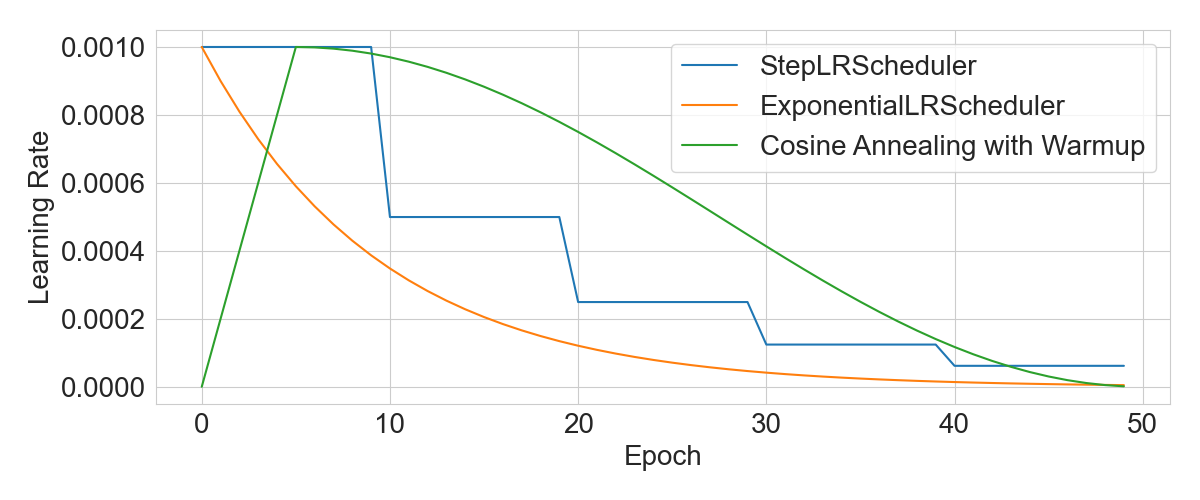
\includegraphics[height=70mm]{./figure/sec3/lr_scheduler.png}
    \caption{スケジューラによる学習率の変化}
    \label{sec3:fig:lr_scheduler}
\end{figure}

\subsubsection{誤差逆伝播法}
\label{sec3:sec:backpropagation}
誤差逆伝播法は,DNNの各重みについての損失関数の勾配を,出力から入力へと遡る方向に計算するアルゴリズムである.ここでは例として,全結合層と活性化関数のみからなる$\numUpper_{\text{layer}}$層のDNNを構築し,ミニバッチ勾配降下法によって最適化する場面を考える\cite{higham2019deep}.

まず,$\weightLower_{p, q}^{n} \in \realSet$を$n - 1$層目の$p$番目のニューロンから$n$層目の$q$番目のニューロンに割り当てられた重み,$b_{p}^{n} \in \realSet$を$n$層目の$p$番目のニューロンに割り当てられたバイアスとすると,$n$層目の$p$番目のニューロンにおける出力$a_{p}^{n} \in \realSet$は,
\begin{equation}
    \label{sec3:eq:output_before_act}
    a_{p}^{n} = b_{p}^{n} + \sum_{q = 1}^{\dimUpper_{n - 1}} \weightLower_{q, p}^{n} o_{q}^{n - 1}
\end{equation}
で与えられる.ここで,$\dimUpper_{n - 1}$は$n - 1$層目の全結合層の次元(総ニューロン数),$o_{q}^{n - 1} \in \realSet$は$n - 1$層目の$q$番目のニューロンにおける出力$a_{q}^{n - 1}$に活性化関数$\phi$を適用した結果を表す.すなわち,
\begin{equation}
    o_{q}^{n - 1} = \phi\lr{a_{q}^{n - 1}}
\end{equation}
である.例外として,各$i \in \mathcal{I}$に対し,$\bm{o}^{0} = \bm{x}_{i}$とする.また,$\dimUpper_{0} = \dimUpper_{\text{in}}, \dimUpper_{N_{\text{layer}}} = \dimUpper_{\text{out}}$とする.ここで,式~\eqref{sec3:eq:output_before_act}に対し,$w_{0, p}^{n} = b_{p}^{n}$,$o_{0}^{n - 1} = 1$とおけば,
\begin{equation}
    \label{sec3:eq:output_before_act_2}
    a_{p}^{n} = b_{p}^{n} + \sum_{q = 1}^{\dimUpper_{n - 1}} w_{q, p}^{n} o_{q}^{n - 1}
    = \sum_{q = 0}^{\dimUpper_{n - 1}} w_{q, p}^{n} o_{q}^{n - 1}
\end{equation}
と整理できる.この時,
\begin{align}
    \pdv{\mathcal{\lossFuncUpper}\lr{\bm{\weightAndBias}; \mathcal{\indexUpper}}}{w_{p, q}^{n}} & = \pdv{w_{p, q}^{n}} \lr{\frac{1}{|\mathcal{\indexUpper}|} \sum_{\indexLower \in \mathcal{\indexUpper}} \lossFuncUpper\lr{\bm{\outputLower}_{\indexLower}, f\lr{\bm{\inputLower}_{\indexLower}; \bm{\weightAndBias}}}} \\
                                                                                                & = \frac{1}{|\mathcal{\indexUpper}|} \sum_{\indexLower \in \mathcal{\indexUpper}} \pdv{\lossFuncUpper\lr{\bm{\outputLower}_{\indexLower}, f\lr{\bm{\inputLower}_{\indexLower}; \bm{\weightAndBias}}}}{w_{p, q}^{n}}     \\
                                                                                                & = \frac{1}{|\mathcal{\indexUpper}|} \sum_{\indexLower \in \mathcal{\indexUpper}} \pdv{\lossFuncUpper_{\indexLower}}{w_{p, q}^{n}}
\end{align}
となる.ここで,$\lossFuncUpper\lr{\bm{\outputLower}_{\indexLower}, f\lr{\bm{\inputLower}_{\indexLower}; \bm{\weightAndBias}}} = \lossFuncUpper_{\indexLower}$とおいた.この時,各$n \in \{1, \ldots, N_{\text{layer}}\}$に対し,
$\pdv*{\lossFuncUpper_{\indexLower}}{w_{p, q}^{n}}$は式\eqref{sec3:eq:output_before_act_2}を用いて,
\begin{align}
    \pdv{\lossFuncUpper_{\indexLower}}{w_{p, q}^{n}} & = \pdv{\lossFuncUpper_{\indexLower}}{a_{q}^{n}} \pdv{a_{q}^{n}}{w_{p, q}^{n}}                \\
                                                     & = \delta_{q}^{n} \pdv{w_{p, q}^{n}} \lr{\sum_{r = 0}^{D_{n - 1}} w_{r, q}^{n} o_{r}^{n - 1}} \\
                                                     & = \delta_{q}^{n} o_{p}^{n - 1}
\end{align}
となる.ここで,$\pdv*{\lossFuncUpper_{\indexLower}}{a_{q}^{n}} = \delta_{q}^{n}$とおいた.このとき,最終層($n = \numUpper_{\text{layer}}$)の重みの場合,
\begin{align}
    \pdv{L_{\indexLower}}{w_{p, q}^{\numUpper_{\text{layer}}}} & = \delta_{q}^{\numUpper_{\text{layer}}} o_{p}^{\numUpper_{\text{layer}} - 1}                                                                                                                                                                                                           \\
                                                               & = o_{p}^{\numUpper_{\text{layer}} - 1} \pdv{L_{i}}{a_{q}^{\numUpper_{\text{layer}}}}                                                                                                                                                                                                   \\
                                                               & = o_{p}^{\numUpper_{\text{layer}} - 1} \pdv{\lossFuncUpper\lr{\bm{\outputLower}_{\indexLower}, f\lr{\bm{\inputLower}_{\indexLower}; \bm{\weightAndBias}}}}{a_{q}^{\numUpper_{\text{layer}}}}                                                                                           \\
                                                               & = o_{p}^{\numUpper_{\text{layer}} - 1} \pdv{\lossFuncUpper\lr{\bm{\outputLower}_{\indexLower}, \phi\lr{\bm{a}^{\numUpper_{\text{layer}}}}}}{a_{q}^{\numUpper_{\text{layer}}}}                                                                                                          \\
                                                               & = o_{p}^{\numUpper_{\text{layer}} - 1} \lr{\nabla_{\phi\lr{\bm{a}^{\numUpper_{\text{layer}}}}} \lossFuncUpper\lr{\bm{\outputLower}_{\indexLower}, \phi\lr{\bm{a}^{\numUpper_{\text{layer}}}}}}^\top \pdv{\phi\lr{\bm{a}^{\numUpper_{\text{layer}}}}}{a_{q}^{\numUpper_{\text{layer}}}} \\
                                                               & = o_{p}^{\numUpper_{\text{layer}} - 1} \pdv{\lossFuncUpper\lr{\bm{\outputLower}_{\indexLower}, \phi\lr{\bm{a}^{\numUpper_{\text{layer}}}}}}{\phi\lr{a_{q}^{\numUpper_{\text{layer}}}}} \phi'\lr{a_{q}^{\numUpper_{\text{layer}}}}
\end{align}
となる.これは,入力から出力を計算する順伝搬で得られた値のみに依存するから,直ちに計算可能であることがわかる.一方,最終層以外($1 \le n < \numUpper_{\text{layer}}$)の重みの場合,
\begin{align}
    \pdv{L_{\indexLower}}{w_{p, q}^{n}} & = \delta_{q}^{n} o_{p}^{n - 1}                                                                                                            \\
                                        & = o_{p}^{n - 1} \pdv{L_{i}}{a_{q}^{n}}                                                                                                    \\
                                        & = o_{p}^{n - 1} \sum_{r = 0}^{D_{n + 1}} \pdv{L_{\indexLower}}{a_{r}^{n + 1}} \pdv{a_{r}^{n + 1}}{a_{q}^{n}}                              \\
                                        & = o_{p}^{n - 1} \sum_{r = 0}^{D_{n + 1}} \delta_{r}^{n + 1} \pdv{a_{q}^{n}} \lr{\sum_{s = 0}^{D_{n}} w_{s, r}^{n + 1} o_{s}^{n}}          \\
                                        & = o_{p}^{n - 1} \sum_{r = 0}^{D_{n + 1}} \delta_{r}^{n + 1} \pdv{a_{q}^{n}} \lr{\sum_{s = 0}^{D_{n}} w_{s, r}^{n + 1} \phi\lr{a_{s}^{n}}} \\
                                        & = o_{p}^{n - 1} \sum_{r = 0}^{D_{n + 1}} \delta_{r}^{n + 1} w_{q, r}^{n + 1} \phi'\lr{a_{q}^{n}}                                          \\
                                        & = o_{p}^{n - 1} \phi'\lr{a_{q}^{n}} \sum_{r = 0}^{D_{n + 1}} \delta_{r}^{n + 1} w_{q, r}^{n + 1}
\end{align}
となる.これは,順伝搬時には計算されない$\delta_{r}^{n + 1}$に依存しているから,$n + 1$層目についての勾配計算を先に行う必要があることがわかる.従って,最終層のみ直ちに勾配を計算可能であり,それ以外の層は自身の次の層に依存しているから,出力から入力へとDNNを遡る方向に計算する,誤差逆伝播法が効率の良いアルゴリズムだと言える.

\subsubsection{学習の安定化}
DNNの学習は勾配降下法によって行われるが,ここで勾配が大きくなりすぎると重みの更新幅が過剰に大きくなり,学習が不安定になる可能性がある.これに対して,Gradient Clippingが有効である.これは,
\begin{equation}
    \nabla_{\bm{\weightAndBias}} \mathcal{\lossFuncUpper}\lr{\bm{\weightAndBias}; \mathcal{I}} \gets \frac{c}{\max \{\lrTwoNorm{\nabla_{\bm{\weightAndBias}} \mathcal{\lossFuncUpper}\lr{\bm{\weightAndBias}; \mathcal{I}}}, c\}} \nabla_{\bm{\weightAndBias}} \mathcal{\lossFuncUpper}\lr{\bm{\weightAndBias}; \mathcal{I}}
\end{equation}
で与えられる.ここで,$c \in \lr{0, \infty}$は勾配のL2ノルムに対する閾値である.

また,近年は数億単位のパラメータを持つ大規模なモデルも提案されており,こういった規模間のモデルを構築して学習する場合,それ相応のメモリが必要になる.マシンのスペックに対し,バッチサイズを十分小さくすれば基本的に学習は可能であるが,これは各データのノイズの影響が強くなるため,学習を不安定にする要因となる.これに対し,Gradient Accumulationが有効である.Gradient Accumulationは,小さなバッチサイズで計算した勾配を複数イテレーションに渡って累積し,設定したイテレーション数ごとに重みの更新を行う手法である.累積される勾配を$\bm{g}_{\text{accum}}$とすると,この更新は
\begin{equation}
    \bm{g}_{\text{accum}} \gets \bm{g}_{\text{accum}} + \nabla_{\bm{\weightAndBias}} \mathcal{\lossFuncUpper}\lr{\bm{\weightAndBias}_{\iter - 1}; \mathcal{I}_{\iter}}
\end{equation}
で与えられる.ここで,設定した累積回数を$\numUpper_{\text{accum}}$とすると,重み$\bm{\weightAndBias}$の更新は
\begin{equation}
    \bm{\weightAndBias}_{\iter} = \bm{\weightAndBias}_{\iter - 1} - \frac{\learningRate}{\numUpper_{\text{accum}}} \bm{g}_{\text{accum}}
\end{equation}
で与えられる.$\numUpper_{\text{accum}}$回分の勾配を累積した分,重みを更新する際には$1 / \numUpper_{\text{accum}}$倍して平均をとることで,実質的に$\numUpper_{\text{accum}}$倍のバッチサイズにおける学習が可能になる.また,重み更新後は累積した勾配を0にリセットして,次の$\numUpper_{\text{accum}}$回の累積に備える.

\subsubsection{自己教師あり学習}
\label{sec3:sec:ssl}
近年,音声や動画を用いる分野では,自己教師あり学習を事前に行ったモデルを特定の問題にFineTuningする転移学習の有効性が確認されている.自己教師あり学習とは、教師ラベルのないデータから特徴を学習する手法であり、データ自体を利用して擬似的な教師ラベルを生成し、教師あり学習を行う点が特徴である。このアプローチは教師なし学習と類似しているが、教師ラベルを生成して利用する点で教師あり学習に近いといえる。ここでは特に,本研究で用いる自己教師あり学習モデルであるHuBERT\cite{hsu2021hubert},AVHuBERT\cite{shi2022learning}で行われている,Masked Predictionという自己教師あり学習方法について述べる.

Masked Predictionでは,データの一部をマスクした上でモデルに入力し,マスクされた領域をモデルに予測させることで学習を行う.入力データを$\bm{\inputUpper} \in \realSet^{T \times D}$とし,このうちマスクされるインデックスの部分集合を$\mathcal{M} \subset \{ 1, \ldots T \}$とする.この時,マスクされた入力$\bm{X}^{\text{masked}}$の各時刻$t$における値$\bm{x}^{\text{masked}}_{t}$は,
\begin{equation}
    \bm{x}^{\text{masked}}_{t} =
    \begin{cases}
        \bm{x}_{t} & \text{if $t \notin \mathcal{M}$} \\
        \bm{m}     & \text{if $t \in \mathcal{M}$}
    \end{cases}
\end{equation}
である.$\bm{m} \in \realSet^{D}$はマスク専用のベクトルである.ここで,HuBERTでは音声データ,AVHuBERTでは動画データと音声データを扱うが,いずれもクラスタリングによって連続特徴量を離散化し,教師ラベルを作成する.クラスタ数$C$のクラスタリングによって得られる教師ラベルを$\bm{Y} \in \{0, 1\}^{T \times C}$とする.各時刻$t$における教師ラベル$\bm{y}_{t}$は,正解クラスが1,それ以外が0となったOne-hotベクトルである.この時,モデルの予測値$\hat{\bm{Y}} \in \lrClosedInterval{0}{1}^{T \times C}$に対する損失は,
\begin{equation}
    L_{\text{CE-masked}}\lr{\bm{Y}, \hat{\bm{Y}}} =
    - \frac{1}{|\mathcal{M}|} \sum_{t \in \mathcal{M}} \sum_{c = 1}^{C} y_{t, c} \log \lr{\hat{y}_{t, c}}
\end{equation}
で与えられる.すなわち,マスクされた位置に限定したCross Entropy Lossである.この損失関数の値を最小化するためには,未知の情報を正しく穴埋めできるように観測できる情報から特徴抽出を行う必要があるから,最適化されたDNNは音声や動画における文脈的な構造を学習していると考えられる.また,音声認識やVSRでは予測対象がテキストになるため,音声データおよび動画データに対するテキストアノテーションを行う必要がある.これに対し,Masked Predictionはテキストを必要としない学習方法であるから,より多くのリソースを用いた学習が可能になるという利点がある.